\documentclass[a4paper, 11pt]{article}

\usepackage{amsmath}
\usepackage{amssymb}
\usepackage{graphicx}
\graphicspath{ {./images/} }
\usepackage{rotating}
\usepackage{float}

\usepackage[a4paper,
            left=0.6in,
            right=0.6in,
            top=1in,
            bottom=1in]{geometry}

\usepackage{hyperref}
\usepackage{lipsum}

\usepackage{multicol}
\setlength{\columnsep}{0.4cm}

\title{Application of High Dimensional Techniques to House Price Prediction}
\vspace{5pt}

\author{
  Pala, Alessandro\\
  \texttt{alessandro.pala@studenti.unipd.it}
  \and
  Tremaggi, Domenico\\
  \texttt{domenico.tremaggi@studenti.unipd.it}
}
\date{}

\begin{document}

\maketitle
\noindent
\begin{abstract}
We explore regression and regularization techniques to predict house prices based on physical, qualitative, locational, and area features. The best result was achieved with a Generalized Additive Model (GAM), explaining approximately 85\% of the variance. Other methods, including linear regression, Poisson regression with Elastic Net, and Group Lasso, were tested, with similar performance. Results indicate that house prices respond highly and independently to house features, and that such relationship can be both linear or polynomial.
\end{abstract}

\vspace{5pt}

\begin{multicols}{2}

\section{Introduction} \vspace{-7pt}
In order to approach the dataset, we first think about which models and variables can predict real estate prices in the real world, with the constraint of the set of variables given by the dataset. Since we handle a price prediction regression, a fair comparison of linear and non-linear basic models - be them regularized or not - would be multivariate. Hence, we first carry a synthetic application of the following models: multivariate linear model and multivariate Poisson regression with an $\alpha = 0.5$ Elastic Net.

In order to understand the higher bound of possible model performance on the dataset, we train a deep multi-layer linear perceptron and we regularize it with a simple Lasso.
Then, we utilise a Group Lasso regression on two sets of groups of variables that we think may be good predictors of house prices in the real world. The first set of groups uses variables that are usually clustered together by real estate professionals when they do house price estimation. The second set of groups uses clusters of highly statistically correlated (Pearson's $r$) variables(Figure \ref{fig:corrmatplot}). Finally, we run a generalized additive model allowing for up to four degrees of freedom on each numerical variable and compare all results.

Selection for regularized models is carried through with cross-validation.

\section{Dataset} \vspace{-7pt}
The dataset contains real estate property listings, each described by a variety of attributes. Temporal attributes are: the listing date, the year the property was built, and the year of its last renovation. Physical characteristics are: the number of bedrooms and bathrooms, living area size, total lot size, number of floors, basement area, and living area above ground. Scenic qualities are represented by a waterfront view indicator, a view quality rating, an overall condition rating, and an overall grade rating. Locational data instead include zip code, latitude, and longitude. There is also some additional spatial context given by the average living area and lot sizes of the 15 nearest properties.

\subsection{Pre-processing} \vspace{-3pt}
In order to pre-process the data, we first convert the date column into a proper date object by extracting the first 8 characters (in "YYYYMMDD" format). We then replace 0 values in the "yr{\_}renovated" column with NA, treating them as missing data. Duplicate rows are removed based on the id column.
We add new variables in the dataset: total{\_}sqft calculates total area by summing living and basement space, bath{\_}per{\_}bed computes the bathroom-to-bedroom ratio (defaulting to 0 if bedrooms are 0), and total{\_}rooms sums bedrooms and bathrooms. sqft{\_}diff{\_}15 measures the difference between the property’s living area and that of its 15 nearest neighbors, while age{\_}since{\_}reno calculates the property’s age since construction, defaulting to 0 if the year is invalid. (Figure \ref{fig:corrplots})
The first, second, fifteenth and sixteenth columns are dropped since they are analytically irrelevant (date, id, with yr{\_}built and yr{\_}renovated being substituted by "age"). We then scale the features of the data frame.
The price and the non-structural features are extracted as columns 2 to 18 and scaled in the new matrix X, which will be used for the Group Lasso. The price, or target, is stored in a separate vector Y.

\section{Base Models} \vspace{-7pt}
\subsection{Multivariate linear model} \vspace{-3pt}
Multivariate Linear Regression is an extension of linear regression where the goal is to model the relationship between multiple independent variables (also called predictors or features) and a dependent variable (also called the target or response variable). It is used when you have more than one predictor variable that you believe influences the dependent variable.

\subsubsection*{Mathematical equation}
\begin{equation}
Y=\beta_0+\beta_1X_1+\beta_2X_2+\dots+\beta_kX_k+\epsilon
\end{equation}

where:$Y$ is the dependent variable, ($X_1, X_2,\dots,X_k$) are the independent variables, $\beta_0$ is the intercept, ($\beta_1,\beta_2, \dots, \beta_k$) are the coefficients and $\epsilon$ is the error term.\\

\subsubsection*{Experiments}
In our case of interest we use all the the available variables to estimate the house prices, including the artificial ones. The model explains approximately 69\% of the variability in the response variable (Figure \ref{fig:MLRpred}) with many variables exhibiting \( p \)-values < 0.001 and, notably, \textbf{sqft\_living}, \textbf{grade}, and \textbf{waterfront} having particularly high coefficients (Table \ref{tab:mlrcoeffs}). Other metrics, along with the plots (Figure \ref{fig:MLR}), tell us that there's some unwanted moderate-scale variability in the predictions.


\subsection{Multivariate GLM with Elastic Net} \vspace{-3pt}
\subsubsection*{The Poisson Distribution}
Poisson regression is based on the Poisson distribution, which describes the probability of a given number of events occurring in a fixed interval of time or space, given the average rate of occurrence.\\
The probability mass function of a Poisson-distributed random variable $Y$ is:
\begin{equation}
P(Y=y)= \frac{\lambda^ye^{-\lambda}}{y!}
\end{equation}
Where: $y$ is the count of events (e.g., number of accidents, number of emails received) and $\lambda$ is the rate of occurrence, which is the expected number of events in the fixed interval.
\subsubsection*{The Poisson Regression Model}
Poisson regression assumes that the logarithm of the expected count (rate) is a linear function of the independent variables.\\
The model is expressed as:
\begin{equation}
\log(\lambda_i)=\beta_0+\beta_1X_1+\beta_2X_2+\dots+\beta_kX_k
\end{equation}
where: ($X_1, X_2,\dots,X_k$) are the indipendent variables, $\beta_0$ is the intercept, ($\beta_1,\beta_2, \dots, \beta_k$) are the regression coefficients.

\subsubsection*{Elastic Net}
In regular linear regression or GLMs, the model can overfit the data if there are many predictors, especially when some predictors are irrelevant or highly correlated, but it can also use some sparsity enforcement, so we applied an Elastic Net regression. This kind of regularization combines $L_1$ and $L_2$ regularizations and applies a penalty to coefficients as to:
\begin{itemize}
    \item Lasso ($L_1$): Shrink some coefficients to
    zero, performing feature selection (Figure 4).
    \item Ridge ($L_2$): Shrink the coefficients (but
    not set them to zero) helping with multi-
    collinearity, which our dataset suffers from.
\end{itemize}
Mathematically, the Elastic Net penalty is given by:
\begin{equation}
\text{Penalty}= \gamma \left[\alpha \sum_{j=1}^k|\beta_j| + \frac{1}{2}(1-\alpha)\sum_{j=1}^k\beta_{j}^{2} \right]
\end{equation} 
where $\gamma$ controls the strength of the regularization (larger $\gamma$ means more regularization), and $\alpha$ controls the balance between Lasso and Ridge.

\subsubsection*{Poisson Regression with Elastic Net}
When you combine Poisson regression with Elastic Net regularization the model becomes:
\begin{equation}
\begin{split}
\log(\lambda_i)&=\beta_0+\beta_1X_1+\beta_2X_2+\dots+\beta_kX_k+ \\
&+\gamma \left[\alpha \sum_{j=1}^k|\beta_j| + \frac{1}{2}(1-\alpha)\sum_{j=1}^k\beta_{j}^{2} \right]
\end{split}
\end{equation}
This means that the objective is to minimize the following loss function:
\begin{equation*}
\text{Loss} = \sum_{i=1}^n \left( -Y_i \log(\lambda_i) + \lambda_i \right) +
\end{equation*}

\begin{equation*}
+ \gamma \left[ \alpha \sum_{j=1}^k |\beta_j| + \frac{1}{2}(1-\alpha) \sum_{j=1}^k \beta_{j}^{2} \right]
\end{equation*}


\subsubsection*{Experiments}
The Poisson regression model had a smooth regularization (Figure \ref{fig:MGLMcoefpath}) and successfully performed variable selection (Table \ref{tab:glmcoefs}) with a relatively normal-looking cross validation plot which resulted in a very large best-lambda value (Figure \ref{fig:MGLMcv}). However, this model's performance was slightly lower than the linear model, explaining 67.5\% of the variance, which means either a wrong distributional assumption or linearity in the relationship in the data (Figure \ref{fig:MGLMperf}). 


\section{Group Lasso} \vspace{-7pt}
The Group Lasso is an extension of the classical Lasso method applied for regularization and variable selection designed to work with grouped variables, and such a situation is helpful when given variables naturally fall into groups, and we want to choose or discard entire groups of variables simultaneously rather than choosing or dropping individual variables.

The main mathematical goal of the Group Lasso is to do regression by penalizing the sum of the norms of the coefficients in each group. That will induce sparsity at the level of groups, that is, all coefficients in a group will either be shrunk towards zero, or not. Therefore, entire groups of variables are either selected or not.

\subsection{Mathematical Formulation} \vspace{-3pt}
For a given linear regression problem, the model can be represented as:
\begin{equation}
y=X\beta + \epsilon
\end{equation}
where: $y$ is the $n \times 1$ vector of observed responses, $X$ is the $n \times p$ matrix of predictors, $\beta$ is the $p \times 1$ vector of regression coefficient and $\epsilon$ is the error term, assumed to be normally distributed.\\

In ordinary linear regression, we try to minimize the residual squared error: \begin{equation} \min_{\beta}\left (\frac{1}{2n}\lVert y-X\beta\rVert^{2}_{2} \right) 
\end{equation}

In the case of Group Lasso, we add a regularization term to the objective function that penalizes the coefficients in groups. If the variables are divided into $G$ groups, and group $g$ contains $p_{g}$ variables, the Group Lasso penalty is given by: \begin{equation} \lambda \sum_{g=1}^{G}\lVert \beta_{g} \rVert_{2}
\end{equation}

The idea would be: where: $\beta_g$ represents the coefficient corresponding to the $g$-th group of variables, $\lVert \beta_g \rVert_2$ is the euclidean norm of the coefficient vector, $\lambda$ is a regularization parameter that regulates its strength.

Thus, the optimization problem is: \begin{equation}
\min_{\beta}\left (\frac{1}{2n}\lVert y-X\beta\rVert^{2}_{2} + \lambda \sum_{g=1}^{G}\lVert \beta_{g} \rVert_{2}\right)
\end{equation}

\subsection{Experiments} \vspace{-3pt}
The model performeds almost identically (Figure \ref{fig:gglassopred}, \ref{fig:gglassoperf}), and as well as the linear regression, explaining about 60\% of the variability in price. The coefficient path plot shows one easily regularizable fast-descending line, with the others being fairly constant throught lambda (Figure \ref{fig:gglassocoefpath}), a result which we also see if we extract each group's contribution in explaining price after cross validation: in the cross-validation lambda choice (Figure \ref{fig:gglassocv}), no group was brought to zero, even though there are significant differences in group importance for both models, which also says something about the adjusted R-squared.
Each set's most contributing group was almost as doubly important as the others (Figure \ref{fig:gglassocontrib}), so it makes sense to mention them: for the first model (real-life modeling) the most important group was group 1, consisting of physical characteristics; bedrooms, bathrooms, lot size and floors. For the second model (inter-correlated features) the most important group was group 4, consisting of house quality measures and extra features; grade, condition, view, waterfront.


\section{Generalized Additive Model}
\subsection{Mathematical Formulation}

Generalized Additive Models (GAMs) are a flexible class of models that extend GLMs by allowing the relationship between the predictors and the response to be modeled as a sum of smooth, potentially non-linear functions.
The mathematical formulation of a GAM is as follows:

We assume an additive relationship to extend the basis function:

\[
f(x) = \sum_{j=1}^p f_j(x_j),
\]


Each \( f_j(x_j) \) may be estimated via some scatterplot smoother \( S \), such as regression splines, loess, parametric methods, etc.

The general form of the additive model is:

\[
y = \beta + \sum_{j=1}^p f_j(x_j) + \phi,
\]

where \( \beta \) is the intercept, and the functions \( f_j(x_j) \) are estimated by the backfitting algorithm.


The backfitting algorithm estimates \( f_j(x_j) \) iteratively:

1. Initialize: \( \hat{\beta} = \frac{\sum_{i} y_i}{n}, \hat{f}_j = 0 \).
2. For each \( j \), update \( \hat{f}_j(x_j) \) using the smoother \( S \):

\[
\hat{f}_j(x_j) \leftarrow S \left( y - \hat{\beta} - \sum_{k \neq j} \hat{f}_k(x_k) \right).
\]



The model is fitted by iteratively smoothing:

\[
y = f_1(x_1) + \cdots + f_p(x_p) + \phi.
\]

Each function \( f_j(x_j) \) is updated in turn, based on the current estimates of the other functions.




\subsection{Experiments}
The firs result of the model is the distribution of the residuals, which exhibits a large range and confirms the presence of outliers in the data, with the IQR going from $-56,686$ to $52,102$ (Table \ref{tab:gamanova}). The model is good at capturing the variance in the data, although and looking at the local scoring process we see a lack of iterations, which means model convergence with no need of further refinements.

The ANOVA table for parametric effects shows that most variables have statistically significant effects on price and, surprisingly, baths per bed (previously significant) being the only one not reaching a satisfactory p-value. The ANOVA table for nonparametric effects (Table \ref{tab:gamanovanonparametric}) shows similar results with all variables being important to predict the price.

Zooming out and looking at the model's general performance, we see that this is the most successful model, explaining circa 85\% of the variability in price, and its MSE being less than half of the previous models' MSE (Figure \ref{fig:gamperf}). By looking at the plots, we can notice that even though many features were best fitted with polynomially, most of them still retained linearity (Figure \ref{fig:gam}). We also see that , just like in the other models, there's some heteroskedasticity, with models specifically struggling with very large values of price (which are also rare). 


\section{Neural Network} \vspace{-7pt}
We finally train a deep neural network in order to have an estimate of the best possible result in any linear statistical context and, most of all, to understand if our choice of models was insufficient.\\
We kept the architecture neither too deep nor too shallow (Figure \ref{fig:NN}) given the medium number of features. We see very clearly that the network uses the features of the dataset to predict extremely well (Figure \ref{fig:NNpred}) and with no overfitting (Figure \ref{fig:traintestloss}). The goal of this small experiment was also to satiate any doubt about the dataset being "corrupted," and that any model could somehow suffer from problems. Indeed, the dataset is not corrupted.

\section{Conclusion} \vspace{-7pt}
\noindent
As shown by the GAM, house prices are not static and respond highly to all sorts of house features, both physical, such as the number of bedrooms or the square feet of the living area, and locational, such as the zipcode or the neighborhood quality. Grouping such features either by mimicking real life statistical groups or according to their inter-correlation did not produce better results than simple models. The latter, if compared to the GAM, seem to highlight that they ignore some variables because they don't capture more complex nonlinear effects, captured instead by the GAM. 
\end{multicols}


\pagebreak
\appendix

\section{Visualization}
 \vspace{7pt}

\begin{figure}[H]
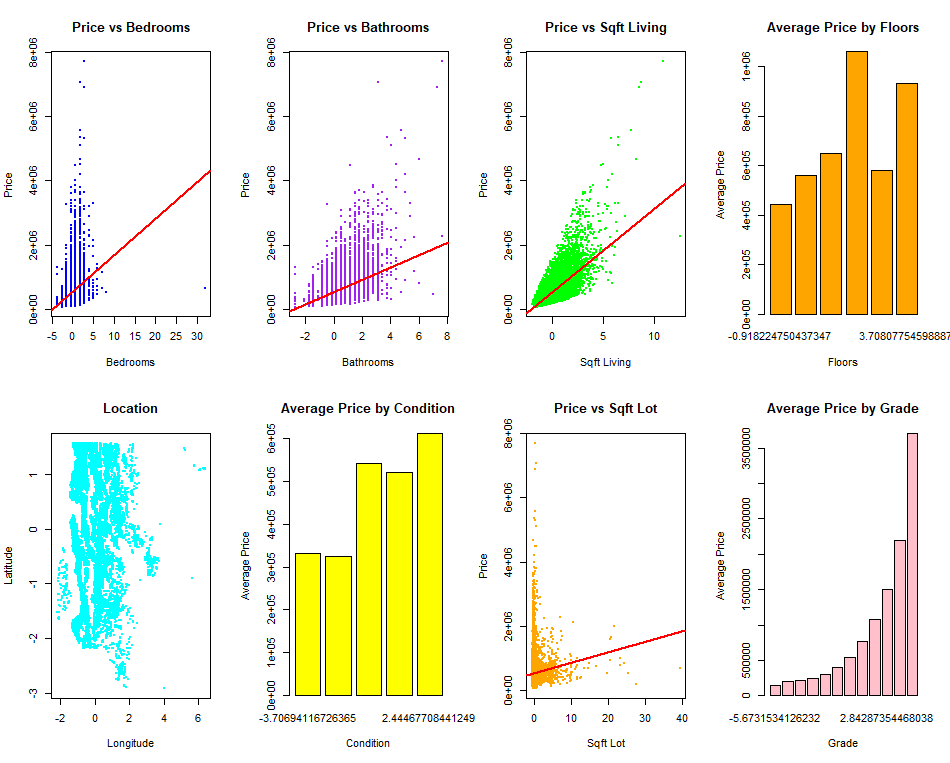
\includegraphics[scale=0.7]{eda}
\centering
\caption{Some simple EDA}
\label{fig:eda}
\end{figure}

\begin{figure}[h]
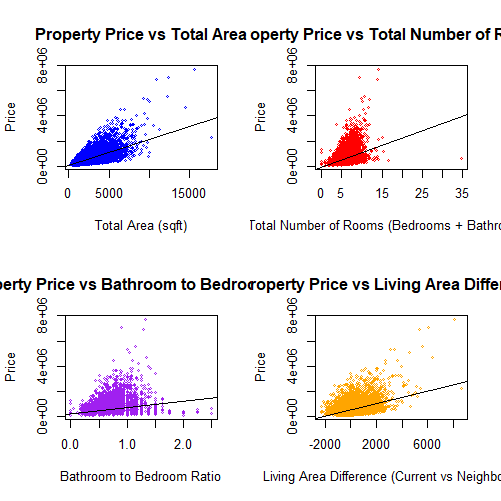
\includegraphics[scale=0.5]{corrplots}
\centering
\caption{How price behaves with aggregated variables}
\label{fig:corrplots}
\end{figure}

\begin{figure}[H]
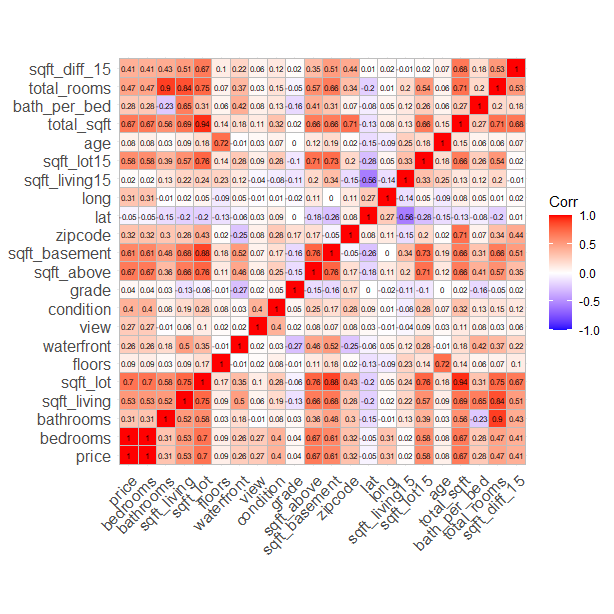
\includegraphics[scale=0.8]{corrmatplot}
\centering
\caption{Correlation matrix to pick groups in the second set of Group Lasso}
\label{fig:corrmatplot}
\end{figure}



\section{Regressions}

\begin{figure}[H]
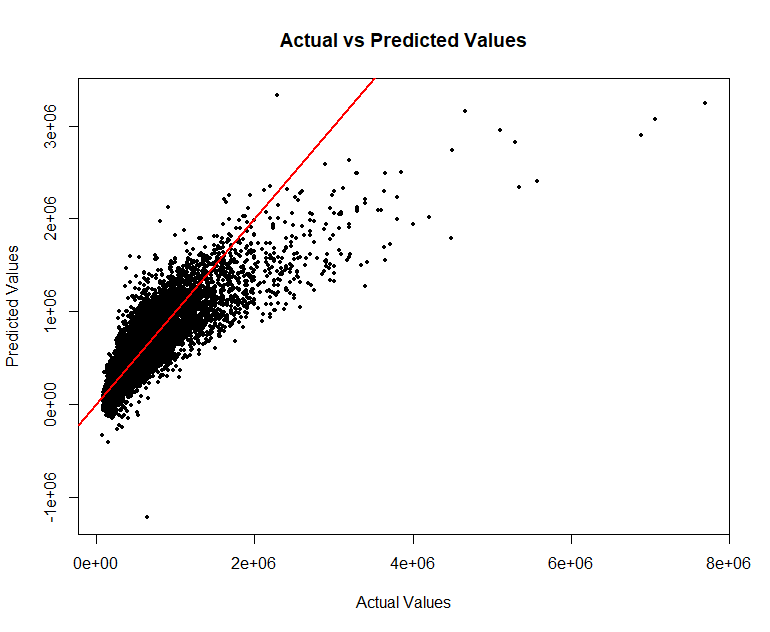
\includegraphics[scale=0.55]{MLRpred}
\centering
\caption{Linear regression actual vs predicted}
\label{fig:MLRpred}
\end{figure}


\begin{figure}[H]
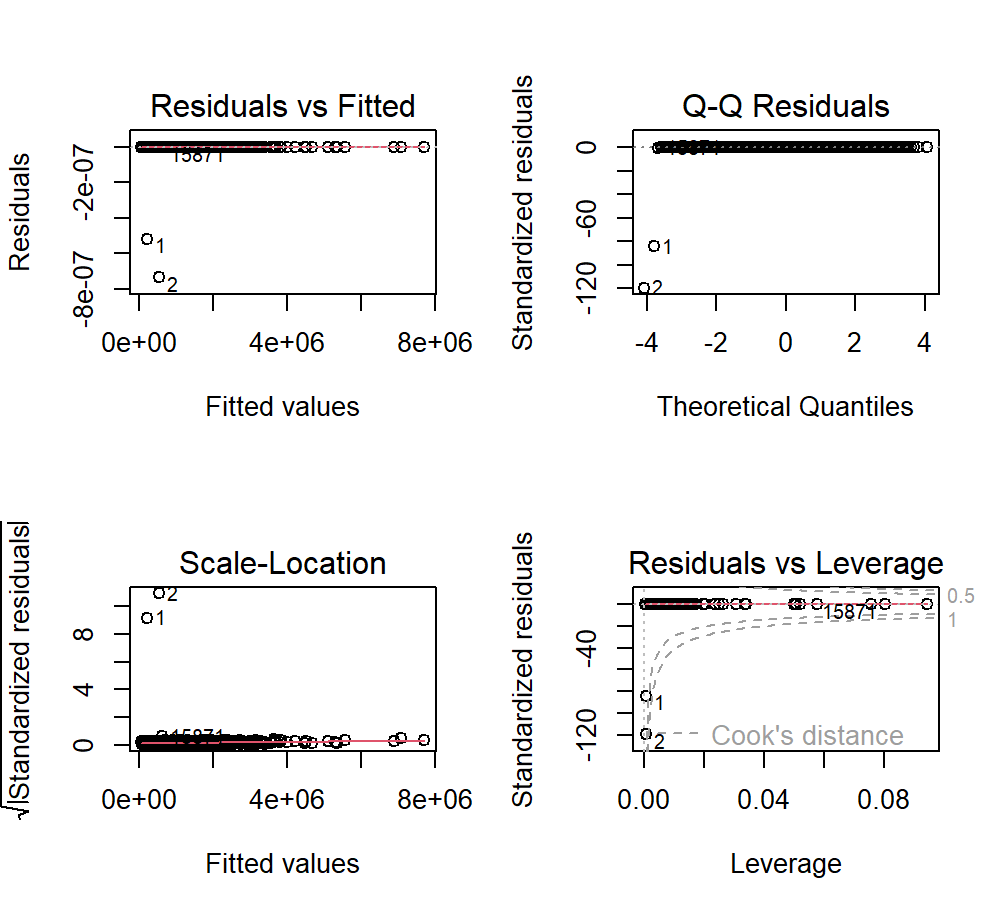
\includegraphics[scale=0.45]{MLR}
\centering
\caption{Multivariate linear regression plot}
\label{fig:MLR}
\end{figure}


\begin{table}[ht]
\centering
\begin{tabular}{|l|r|r|r|r|}
\hline
\textbf{Variable} & \textbf{Estimate} & \textbf{Std. Error} & \textbf{t value} & \textbf{p value} \\
\hline
(Intercept)       & $5.359 \times 10^{5}$  & $1.402 \times 10^{3}$  & $3.821 \times 10^{2}$  & $< 2 \times 10^{-16}$ ***  \\
bedrooms          & $-2.994 \times 10^{4}$ & $1.819 \times 10^{3}$  & $-1.647 \times 10^{1}$ & $< 2 \times 10^{-16}$ ***  \\
bathrooms         & $1.461 \times 10^{4}$  & $2.845 \times 10^{3}$  & $5.134 \times 10^{0}$  & $2.87 \times 10^{-7}$ ***   \\
sqft\_living      & $1.471 \times 10^{5}$  & $4.093 \times 10^{3}$  & $3.594 \times 10^{1}$  & $< 2 \times 10^{-16}$ ***  \\
sqft\_lot         & $5.957 \times 10^{3}$  & $2.023 \times 10^{3}$  & $2.945 \times 10^{0}$  & $3.23 \times 10^{-3}$ **    \\
floors            & $3.164 \times 10^{3}$  & $1.995 \times 10^{3}$  & $1.586 \times 10^{0}$  & 0.113          \\
waterfront        & $6.047 \times 10^{5}$  & $1.763 \times 10^{4}$  & $3.430 \times 10^{1}$  & $< 2 \times 10^{-16}$ ***  \\
view              & $4.406 \times 10^{4}$  & $1.668 \times 10^{3}$  & $2.641 \times 10^{1}$  & $< 2 \times 10^{-16}$ ***  \\
condition         & $1.827 \times 10^{4}$  & $1.570 \times 10^{3}$  & $1.164 \times 10^{1}$  & $< 2 \times 10^{-16}$ ***  \\
grade             & $1.073 \times 10^{5}$  & $2.572 \times 10^{3}$  & $4.174 \times 10^{1}$  & $< 2 \times 10^{-16}$ ***  \\
sqft\_above       & $1.900 \times 10^{4}$  & $3.712 \times 10^{3}$  & $5.119 \times 10^{0}$  & $3.10 \times 10^{-7}$ ***   \\
sqft\_basement    & NA          & NA         & NA         & NA             \\
zipcode           & $-2.920 \times 10^{4}$ & $1.798 \times 10^{3}$  & $-1.624 \times 10^{1}$ & $< 2 \times 10^{-16}$ ***  \\
lat               & $8.648 \times 10^{4}$  & $1.514 \times 10^{3}$  & $5.712 \times 10^{1}$  & $< 2 \times 10^{-16}$ ***  \\
long              & $-3.515 \times 10^{4}$ & $1.878 \times 10^{3}$  & $-1.871 \times 10^{1}$ & $< 2 \times 10^{-16}$ ***  \\
sqft\_living15    & $1.092 \times 10^{4}$  & $2.408 \times 10^{3}$  & $4.535 \times 10^{0}$  & $5.80 \times 10^{-6}$ ***   \\
sqft\_lot15       & $-1.011 \times 10^{4}$ & $2.039 \times 10^{3}$  & $-4.957 \times 10^{0}$ & $7.23 \times 10^{-7}$ ***   \\
age               & $5.985 \times 10^{4}$  & $2.105 \times 10^{3}$  & $2.844 \times 10^{1}$  & $< 2 \times 10^{-16}$ ***  \\
total\_sqft       & NA          & NA         & NA         & NA             \\
bath\_per\_bed    & $2.120 \times 10^{4}$  & $1.931 \times 10^{3}$  & $1.098 \times 10^{1}$  & $< 2 \times 10^{-16}$ ***  \\
total\_rooms      & NA          & NA         & NA         & NA             \\
sqft\_diff\_15    & NA          & NA         & NA         & NA             \\
\hline
\end{tabular}
\caption{Multivariate Linear Regression Data Summary}
\label{tab:mlrcoeffs}
\end{table}


\begin{figure}[H]
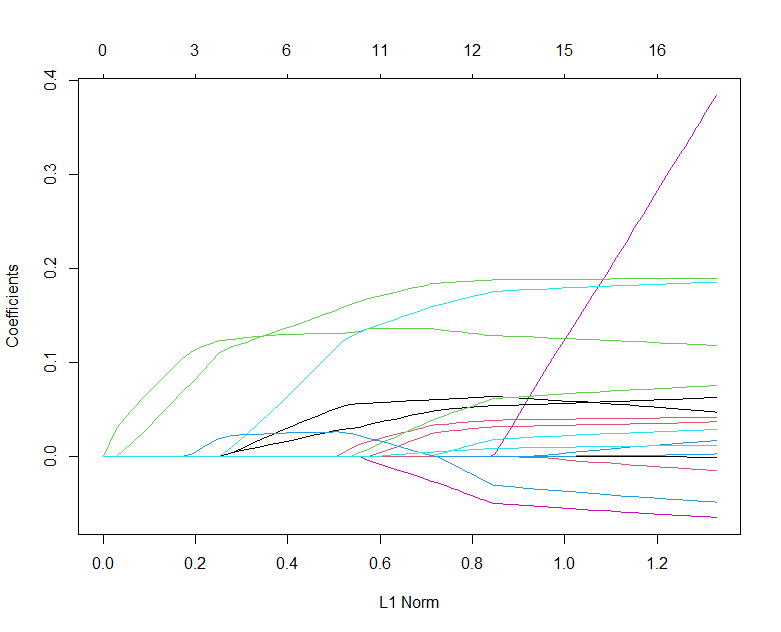
\includegraphics[scale=0.55]{MGLMcoefpath}
\centering
\caption{Multivariate Poisson regression coefficient path}
\label{fig:MGLMcoefpath}
\end{figure}

\begin{figure}[H]
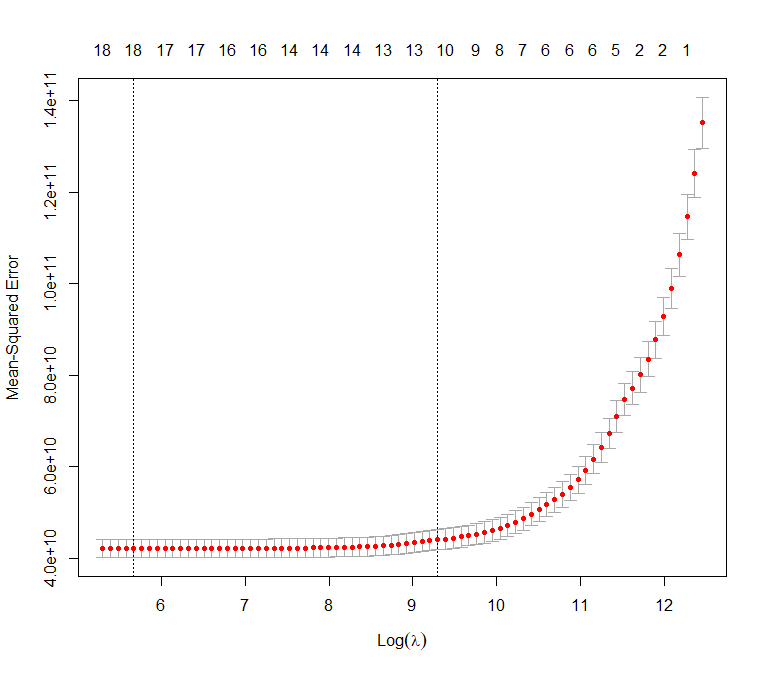
\includegraphics[scale=0.65]{MGLMcv}
\centering
\caption{Cross validation plot for Poisson regression}
\label{fig:MGLMcv}
\end{figure}


\begin{table}[ht] \centering \begin{tabular}{|l | r|} \hline \textbf{Variable} & \textbf{Coefficient} \\ \hline Intercept & 536525.639 \\ Bedrooms & -1009.958 \\ Bathrooms & . \\ Sqft\_Living & 145781.906 \\ Sqft\_Lot & . \\ Floors & . \\ Waterfront & 526574.268 \\ View & 40996.640 \\ Condition & 11319.671 \\ Grade & 109439.811 \\ Sqft\_Above & . \\ Sqft\_Basement & . \\ Zipcode & . \\ Lat & 74933.499 \\ Long & -11647.660 \\ Sqft\_Living15 & 6652.210 \\ Sqft\_Lot15 & . \\ Age & 38344.499 \\ \hline \end{tabular} \caption{Coefficients from the Poisson model} \label{tab:glmcoefs} \end{table}

\begin{figure}[H]
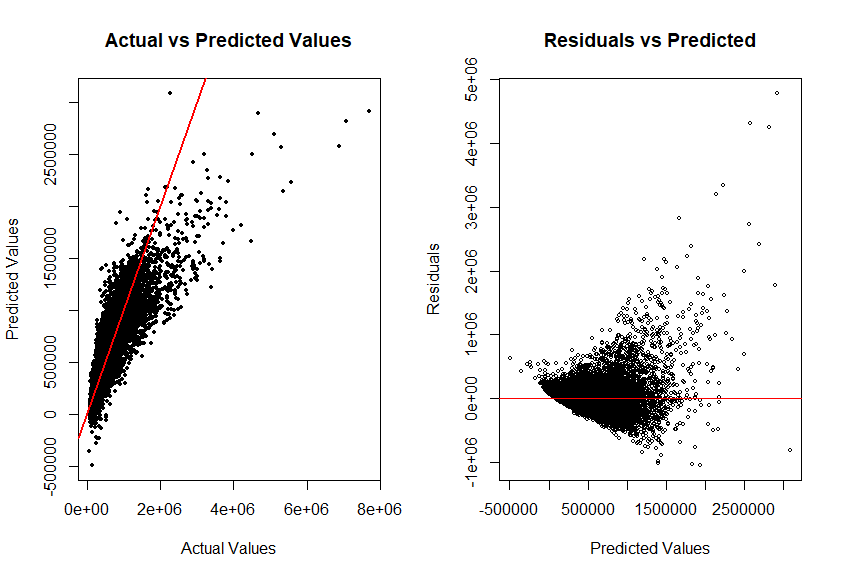
\includegraphics[scale=0.65]{MGLMperf}
\centering
\caption{Poisson regression performance}
\label{fig:MGLMperf}
\end{figure}


\begin{figure}[H]
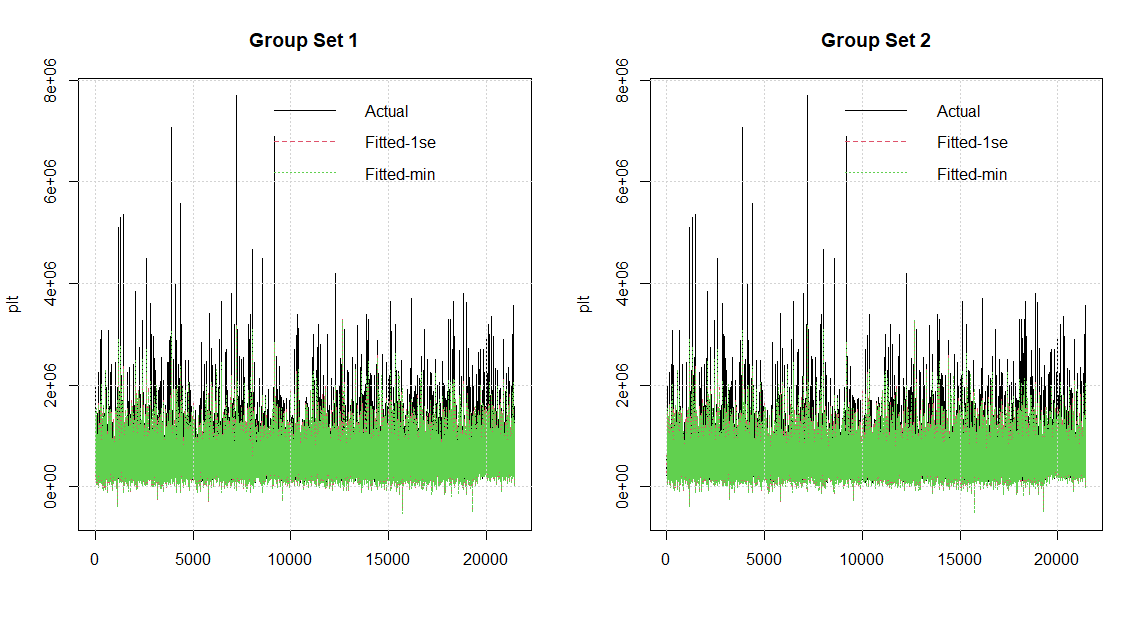
\includegraphics[scale=0.5]{gglassopred}
\centering
\caption{Grouped models predictions}
\label{fig:gglassopred}
\end{figure}

\begin{figure}[H]
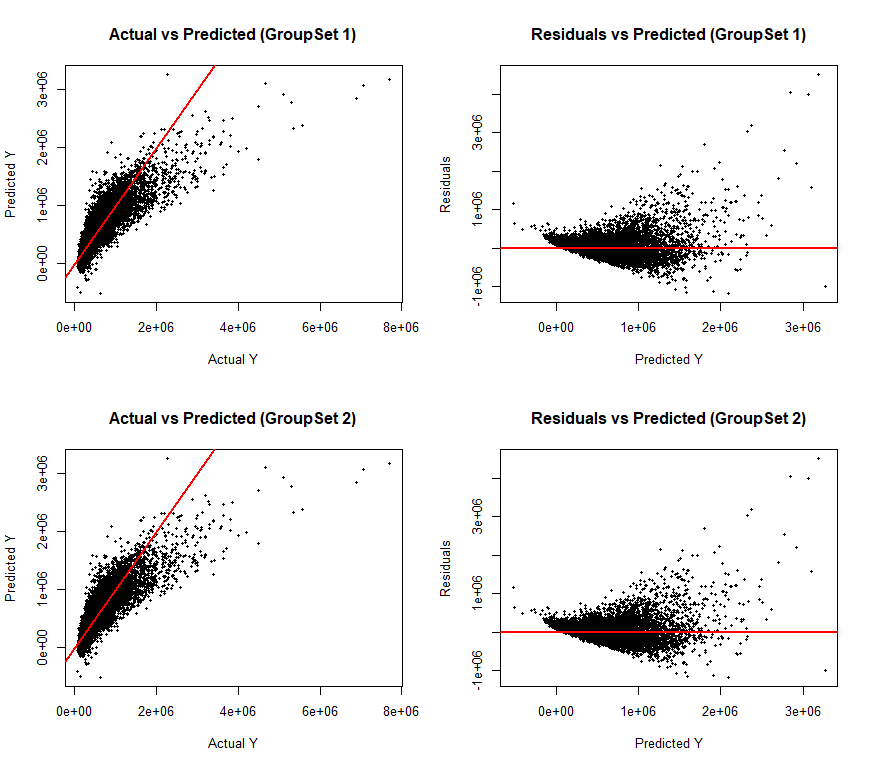
\includegraphics[scale=0.65]{gglassoperf}
\centering
\caption{Grouped models performances(only min lambda)}
\label{fig:gglassoperf}
\end{figure}

\begin{figure}[H]
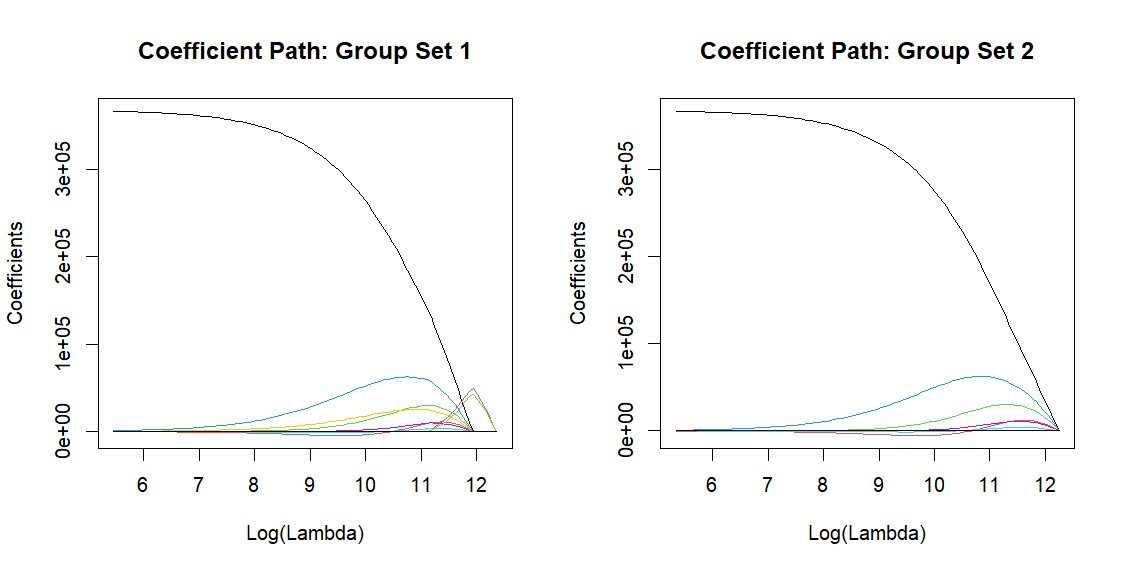
\includegraphics[scale=0.55]{gglassocoefpath}
\centering
\caption{Coefficient path for Group Lasso}
\label{fig:gglassocoefpath}
\end{figure}

\begin{figure}[H]
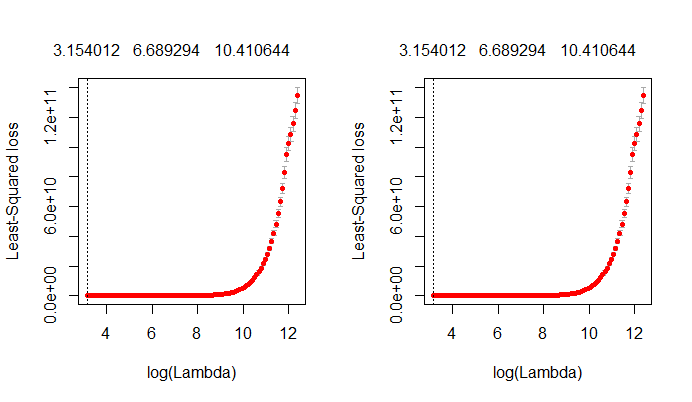
\includegraphics[scale=0.55]{gglassocv}
\centering
\caption{Cross Validation for Group Lasso}
\label{fig:gglassocv}
\end{figure}

\begin{figure}[H]
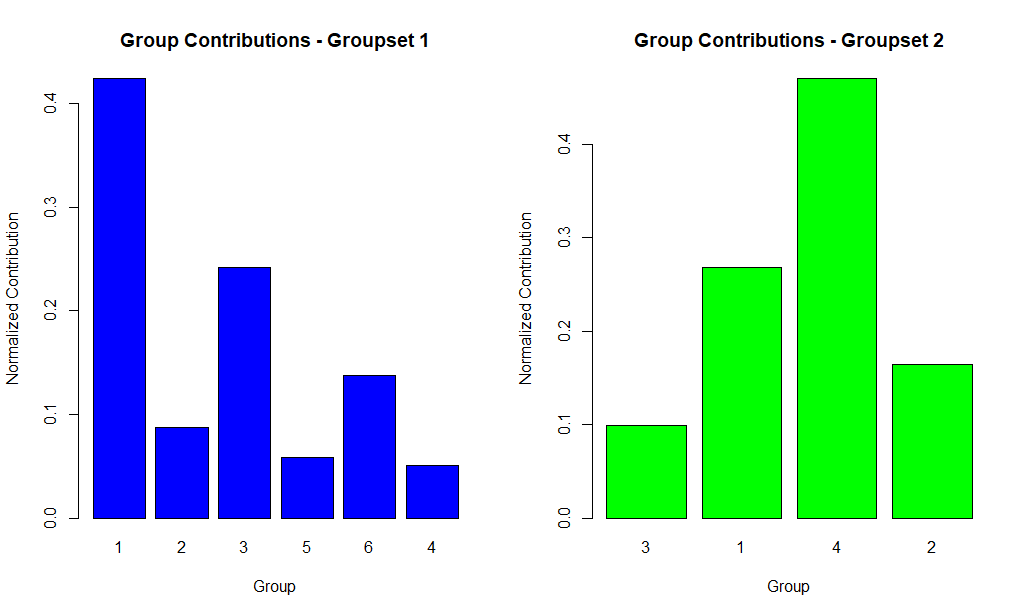
\includegraphics[scale=0.5]{gglassocontrib}
\centering
\caption{Group contribution for gglasso models}
\label{fig:gglassocontrib}
\end{figure}


\begin{figure}[H]
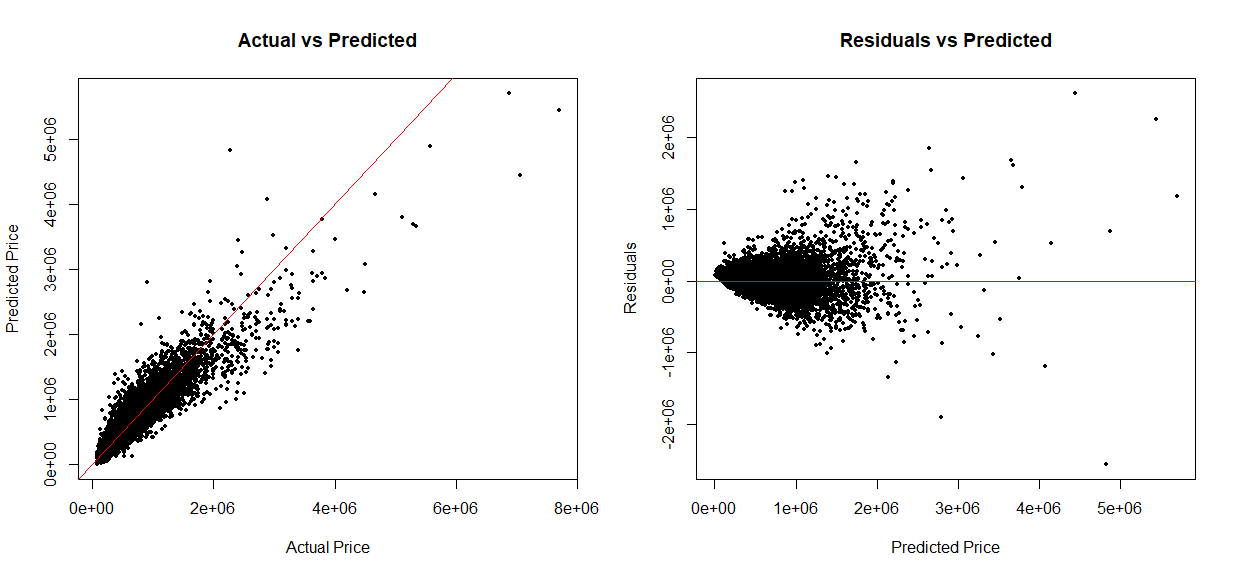
\includegraphics[scale=0.4]{gamperf}
\centering
\caption{GAM performance}
\label{fig:gamperf}
\end{figure}

\begin{figure}[H]
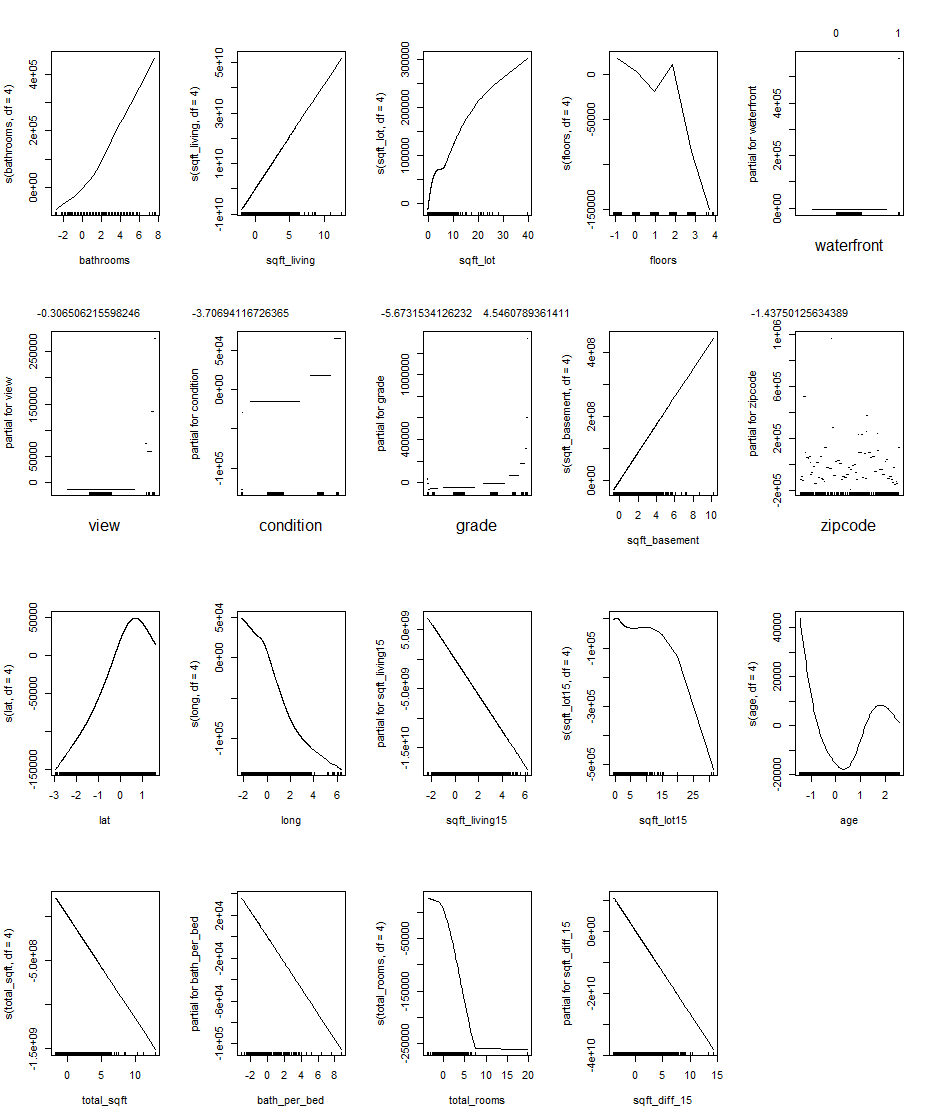
\includegraphics[scale=0.4]{gam}
\centering
\caption{GAM/splines: price vs each feature}
\label{fig:gam}
\end{figure}

\begin{table}[ht]
\centering
\begin{tabular}{|l|r|r|r|r|l|}
\hline
\textbf{Variable} & \textbf{Df} & \textbf{Sum Sq} & \textbf{Mean Sq} & \textbf{F value} & \textbf{P($>$F)} \\
\hline
s(bathrooms, df = 4) & 1 & $8.03 \times 10^{14}$ & $8.03 \times 10^{14}$ & 39053.23 & $< 2.2 \times 10^{-16}$ *** \\
s(sqft\_living, df = 4) & 1 & $5.96 \times 10^{14}$ & $5.96 \times 10^{14}$ & 28967.84 & $< 2.2 \times 10^{-16}$ *** \\
s(sqft\_lot, df = 4) & 1 & $1.51 \times 10^{12}$ & $1.51 \times 10^{12}$ & 73.61 & $< 2.2 \times 10^{-16}$ *** \\
s(floors, df = 4) & 1 & $1.36 \times 10^{11}$ & $1.36 \times 10^{11}$ & 6.61 & 0.0102 * \\
waterfront & 1 & $1.02 \times 10^{14}$ & $1.02 \times 10^{14}$ & 4962.16 & $< 2.2 \times 10^{-16}$ *** \\
view & 4 & $5.78 \times 10^{13}$ & $1.45 \times 10^{13}$ & 702.67 & $< 2.2 \times 10^{-16}$ *** \\
condition & 4 & $1.58 \times 10^{13}$ & $3.96 \times 10^{12}$ & 192.59 & $< 2.2 \times 10^{-16}$ *** \\
grade & 11 & $1.89 \times 10^{14}$ & $1.72 \times 10^{13}$ & 836.48 & $< 2.2 \times 10^{-16}$ *** \\
s(sqft\_basement, df = 4) & 1 & $3.98 \times 10^{12}$ & $3.98 \times 10^{12}$ & 193.72 & $< 2.2 \times 10^{-16}$ *** \\
zipcode & 69 & $4.74 \times 10^{14}$ & $6.86 \times 10^{12}$ & 333.79 & $< 2.2 \times 10^{-16}$ *** \\
s(lat, df = 4) & 1 & $8.43 \times 10^{11}$ & $8.43 \times 10^{11}$ & 40.98 & $1.57 \times 10^{-10}$ *** \\
s(long, df = 4) & 1 & $7.32 \times 10^{11}$ & $7.32 \times 10^{11}$ & 35.58 & $2.49 \times 10^{-9}$ *** \\
sqft\_living15 & 1 & $1.65 \times 10^{12}$ & $1.65 \times 10^{12}$ & 80.44 & $< 2.2 \times 10^{-16}$ *** \\
s(sqft\_lot15, df = 4) & 1 & $2.35 \times 10^{11}$ & $2.35 \times 10^{11}$ & 11.43 & 0.0007 *** \\
s(age, df = 4) & 1 & $4.43 \times 10^{11}$ & $4.43 \times 10^{11}$ & 21.53 & $3.50 \times 10^{-6}$ *** \\
s(total\_sqft, df = 4) & 1 & $3.09 \times 10^{11}$ & $3.09 \times 10^{11}$ & 15.02 & $1.06 \times 10^{-4}$ *** \\
bath\_per\_bed & 1 & $2.05 \times 10^{9}$ & $2.05 \times 10^{9}$ & 0.10 & 0.752 \\
s(total\_rooms, df = 4) & 1 & $5.97 \times 10^{11}$ & $5.97 \times 10^{11}$ & 29.04 & $7.17 \times 10^{-8}$ *** \\
sqft\_diff\_15 & 1 & $5.42 \times 10^{11}$ & $5.42 \times 10^{11}$ & 26.33 & $2.90 \times 10^{-7}$ *** \\
\hline
Residuals & 21299 & $4.38 \times 10^{14}$ & $2.06 \times 10^{10}$ & & \\
\hline
\end{tabular}
\caption{GAM: ANOVA for Parametric Effects}
\label{tab:gamanova}
\end{table}

\begin{table}[ht]
\centering
\begin{tabular}{|l|r|r|l|}
\hline
\textbf{Variable} & \textbf{Npar Df} & \textbf{Npar F} & \textbf{P($>$F)} \\
\hline
s(bathrooms, df = 4) & 3 & 22.99 & $7.44 \times 10^{-15}$ *** \\
s(sqft\_living, df = 4) & 3 & 76.91 & $< 2.2 \times 10^{-16}$ *** \\
s(sqft\_lot, df = 4) & 3 & 21.60 & $5.84 \times 10^{-14}$ *** \\
s(floors, df = 4) & 3 & 24.35 & $9.99 \times 10^{-16}$ *** \\
s(sqft\_basement, df = 4) & 3 & 70.34 & $< 2.2 \times 10^{-16}$ *** \\
s(lat, df = 4) & 3 & 51.48 & $< 2.2 \times 10^{-16}$ *** \\
s(long, df = 4) & 3 & 15.16 & $7.52 \times 10^{-10}$ *** \\
s(sqft\_lot15, df = 4) & 3 & 14.56 & $1.82 \times 10^{-9}$ *** \\
s(age, df = 4) & 3 & 61.05 & $< 2.2 \times 10^{-16}$ *** \\
s(total\_sqft, df = 4) & 3 & 333.48 & $< 2.2 \times 10^{-16}$ *** \\
s(total\_rooms, df = 4) & 3 & 24.54 & $7.77 \times 10^{-16}$ *** \\
\hline
\end{tabular}
\caption{GAM: ANOVA for Nonparametric Effects}
\label{tab:gamanovanonparametric}
\end{table}


\begin{figure}[H]
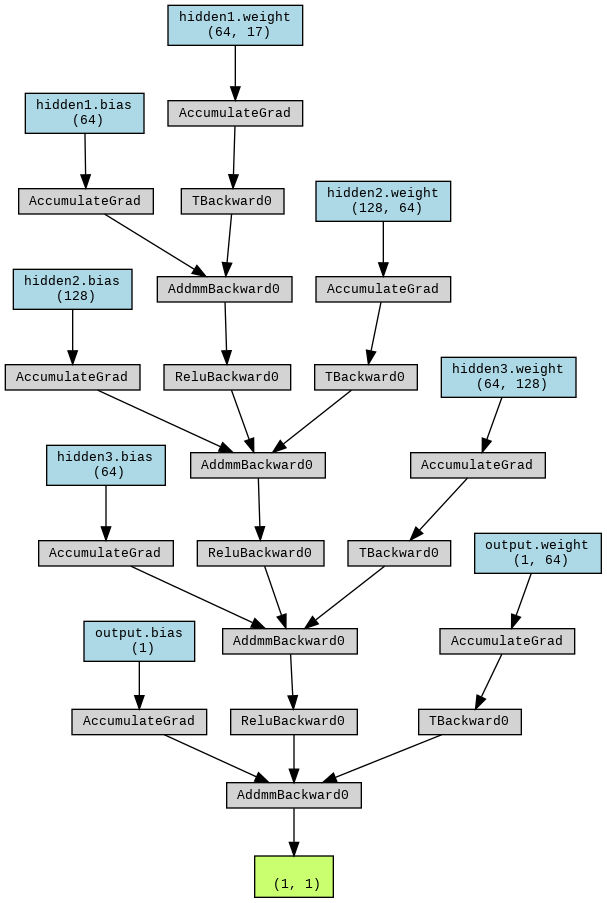
\includegraphics[scale=0.65]{NN}
\centering
\caption{Neural Network architecture}
\label{fig:NN}
\end{figure}

\begin{figure}[H]
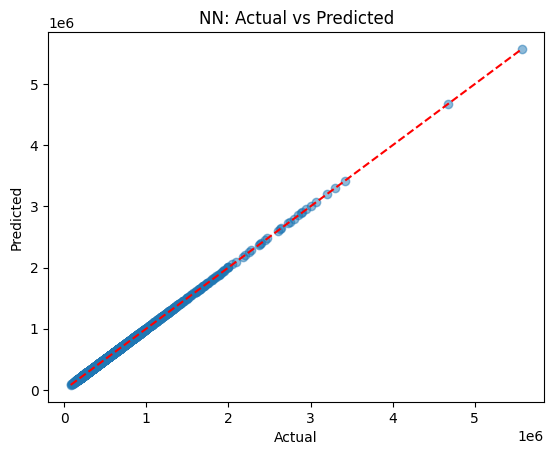
\includegraphics[scale=0.7]{NNpred}
\centering
\caption{Neural Network actual vs predicted}
\label{fig:NNpred}
\end{figure}

\begin{figure}[H]
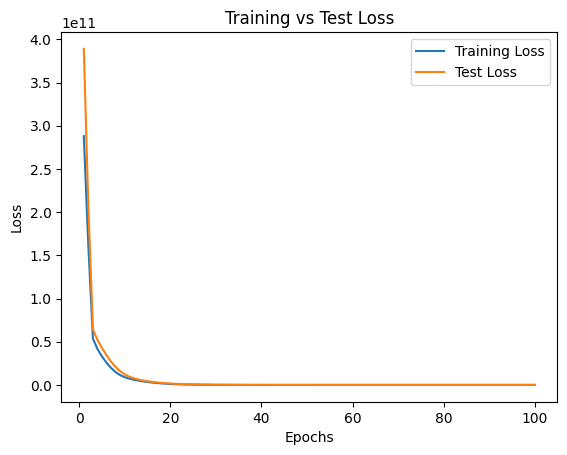
\includegraphics[scale=0.75]{traintestloss}
\centering
\caption{Neural Network training}
\label{fig:traintestloss}
\end{figure}



\end{document}